%%%%%%%%%%%%%%%%%%%%%%%%%%%%%%%%%%%%%%%%%%%%%%%%%%%%%%%%%%%%%%%%%%%%
\section{Cryogenics Instrumentation}
\label{sec:fdsp-cryo-instr} % label used for \ref's from single phase sections.
\label{sec:fddp-cryo-instr} % label used for \ref's from dual phase sections.
\label{sec:fdgen-cryo-instr} % label used for \ref's from generic sections.
% Jim G %Carmen

Instrumentation inside the cryostat must ensure that the condition of the \dword{lar} is adequate for operation of the \dshort{tpc}.
This instrumentation includes devices to monitor the impurity level of the argon, e.g., the purity monitors, which provide high-precision electron lifetime measurements,
and gas analyzers to ensure that the levels of atmospheric contamination drop below certain limits during the cryostat purging, cooling and filling.
The cryogenics system operation is monitored by temperature sensors deployed in vertical arrays and at the top and bottom of the detector, providing a 
detailed \threed temperature map that can help to predict the \dword{lar} purity across the entire cryostat. The cryogenics instrumentation also includes \lar level monitors and
a system of internal cameras to help in locating sparks in the cryostat and for overall monitoring of the cryostat interior. 
As mentioned in the introduction, cryogenics instrumentation requires simulation work to identify the proper location for these devices inside the cryostat and
for the coherent analysis of the instrumentation data. 

Figure~\ref{fig:sp-slow-cryo-ports} shows the current map of cryostat ports for the \dword{spmod}, highlighting the ones assigned to instrumentation devices,
as well as the preliminary location for some of these devices. Vertical temperature profilers are located behind the \dwords{apa} ($T_S$) and behind the east end wall ($T_D$).
They are complemented by a coarser \twod grid of sensors at the top and bottom of the cryostat (not shown in the figure). Purity monitors and level meters are planned
in each detector side, behind the two front end walls. Inspection cameras will use some of the multipurpose instrumentation ports, but their exact locations are yet to be decided. 


\begin{dunefigure}[Cryostat ports]{fig:sp-slow-cryo-ports}
{Cryostat ports and preliminary location of some instrumentation devices. }
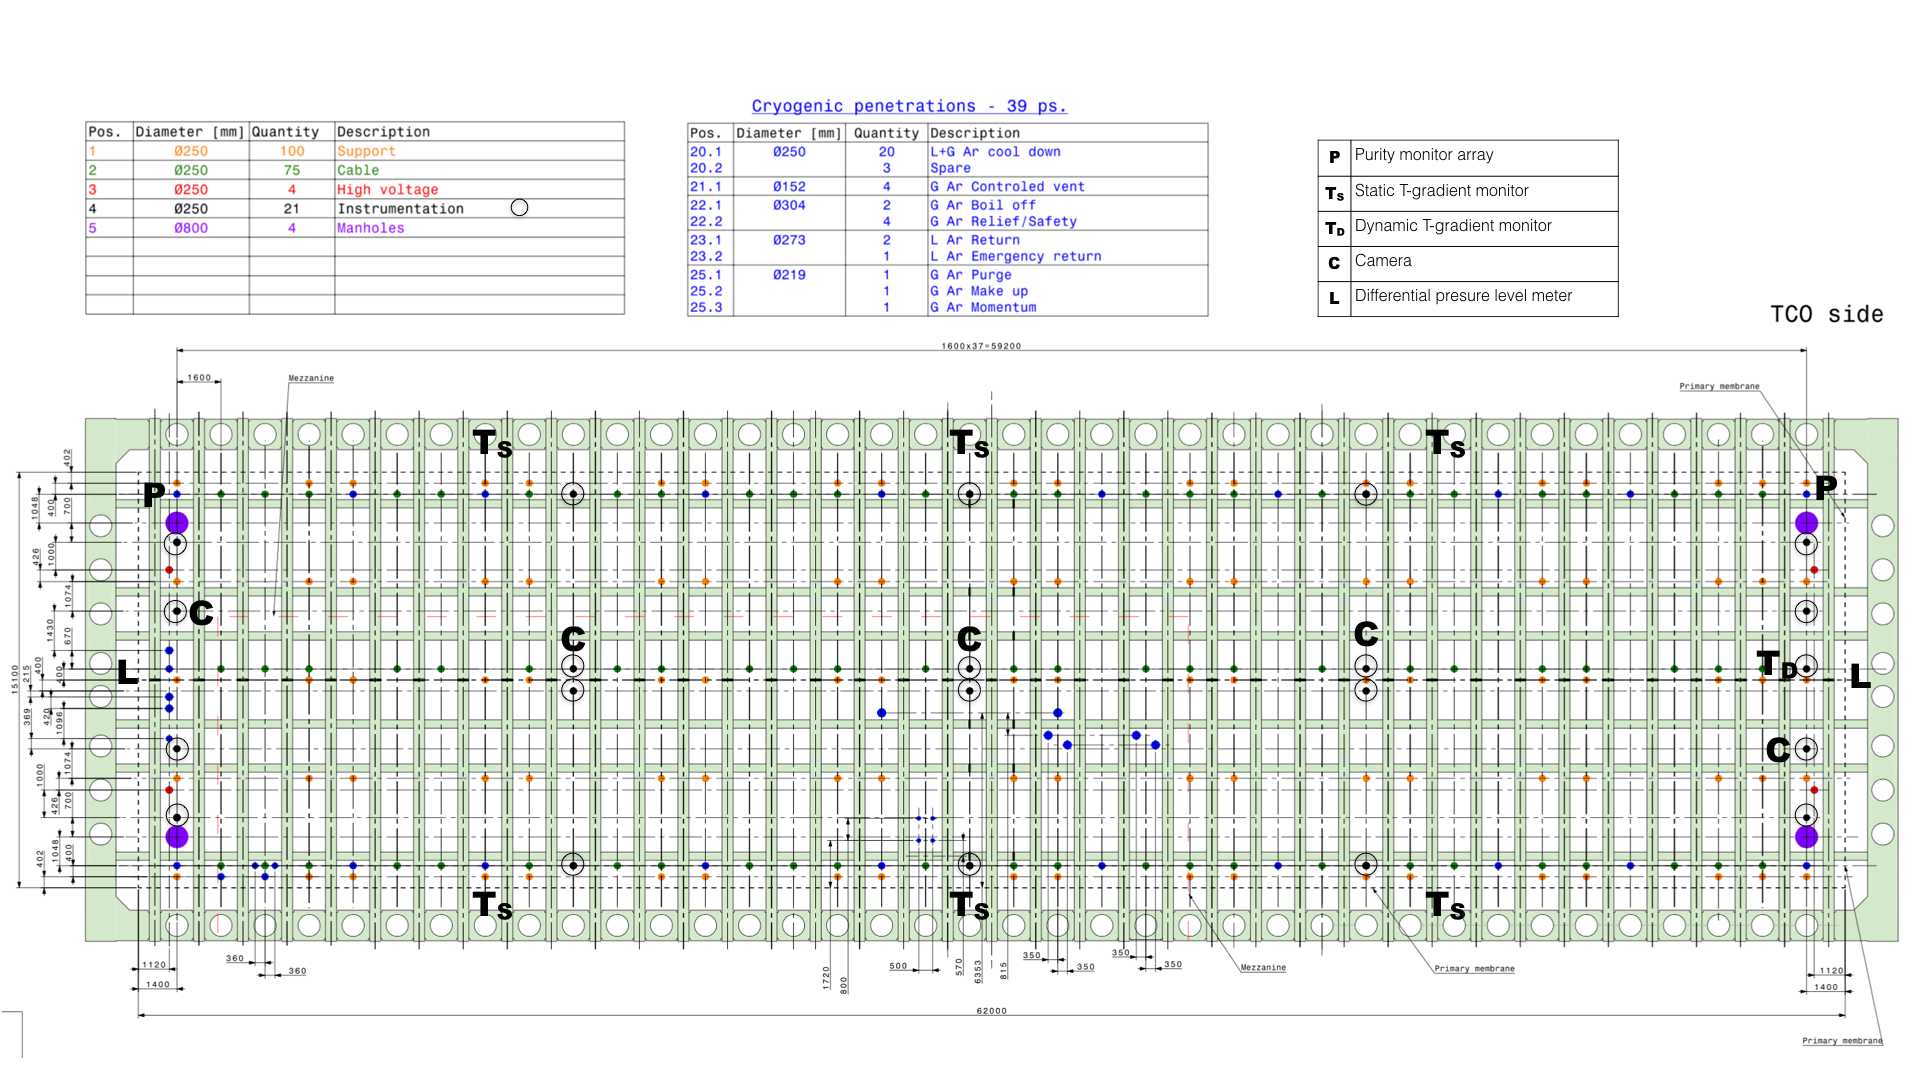
\includegraphics[width=0.95\textwidth]{cisc_cryostat_ports.png}
\end{dunefigure}


